\documentclass[12pt,consuni]{uftpibic}

\usepackage[alf]{abntex2cite}
%\renewcommand{\backrefpagesname}{}
%\renewcommand{\backref}{}
\renewcommand*{\backrefalt}[4]{}
%-------------------------------------------------------------------------------------------------------------------------%
% Endereço Institucional
%-------------------------------------------------------------------------------------------------------------------------%
\address{109 Norte, Av. Ns 15, ALCNO 14, Bl 04, Sala 207}
\cep{77001-090}
\phone{(63) 3232-8037}
\mail{propesq@uft.edu.br}
\city{Palmas}
%-------------------------------------------------------------------------------------------------------------------------%
% Dados do Projeto
%-------------------------------------------------------------------------------------------------------------------------%
\title{RUTI - RASTREAMENTO URBANO DE TRANSPORTE INTEGRADO – PROCESSO NÚMERO 1966/2017}
\advisor{Prof.}{Tiago da Silva}{Almeida}{Ms.}
\author{Matheus Aguiar}{Fagundes}
\campus{Campus Universitário de Palmas -- CUP}
\department{Ciência da Computação}
\local{Campus Universitário de Palmas -- CUP, Bloco III, Sala 09}
\area{Ciências Exatas e da Terra}
\financiamento{}
\grupo{GCC -- Grupo de Computação Cientifica}
\keyword{IoT}
\keyword{Transporte Urbano}
\keyword{Rastreamento}
\keyword{Sistemas Embarcados}
\keyword{Transporte Urbano}
\keyword{Rastreamento}
\keyword{Sistemas Embarcados}
\equipeexecutora{\bf Tiago da Silva Almeida}{\bf Coordenador}
\equipeexecutora{Rafael Lima de Carvalho}{Professor Pesquisador}
\equipeexecutora{Warley Gramacho da Silva}{Professor Pesquisador}
\equipeexecutora{Leonardo Rezende Costa}{Aluno}
\equipeexecutora{Matheus Aguiar Fagundes}{Aluno}
%-------------------------------------------------------------------------------------------------------------------------%
% Para evitar a quebra automática dos Capítulos, descomentar abaixo
%-------------------------------------------------------------------------------------------------------------------------%
%\makeatletter
%\patchcmd{\chapter}{\if@openright\cleardoublepage\else\clearpage\fi}{}{}{}
%\makeatother
%-------------------------------------------------------------------------------------------------------------------------%
\begin{document}

\maketitle


\chapter{Introdução}

Grandes centros urbanos trazem grandes desafios à gestão na prestação de serviços de qualidade à população. Um desses desafios é o controle de tráfego devido ao tamanho da frota em grandes centros. Atualmente vivemos uma fase de popularização de projetos que envolvam algum tipo de automação eletrônica. Isso é possível devido aos baixos custos e integração de grande variedades de circuitos acoplados (ou dentro do mesmo encapsulamento, os chamados System-on-Chip ou somente SoC), trazendo simplicidade na construção de sistemas automáticos. Logo, surgiu uma linha de pesquisa, chamada Internet of Things (IoT), em conjunto com a também simplificada área de desenvolvimento Web. A aplicabilidade da metodologia IoT é bastante diversa, podendo ser aplicada também ao controle de tráfego urbano nas grandes cidades. Assim, o objeto desse projeto é desenvolver uma solução baseada em IoT para gerenciamento de frota urbana, especificamente em transporte coletivo. Nosso objetivo é desenvolver um sistema de rastreamento e controle individual de cada veículo, com geolocalização, alimentar uma aplicação web com esses dados e também fornecer informações em tempo real aos usuários. Os dados capturados dos veículos podem ser utilizados para tomada de decisão em relação a melhores rotas, gastos globais com o transporte, etc.. Um grande desafio, e foco do projeto, é a melhor tecnologia de troca de dados entre veículos e a aplicação Web, devido ao custo de equipamento mais seguros e rápidos e a baixa qualidade da infraestrutura existente. Portanto, nossos esforços empenham-se no sistema de coleta e gestão de dados da frota veicular. \citeonline{Al-Qaseemi}

\chapter{Objetivos}


\chapter{Metodologia}

Para o desenvolvimento do projeto serão utilizadas plataformas microcontroladas para gerenciamento da comunicação de dados. Atualmente diversas plataformas baseadas em microcontroladores e SoCs são empregadas em projeto de IoT, e em sua maioria são de código fonte aberto. Por possuir um custo baixo e ampla documentação, escolhemos a plataforma Arduino.

\begin{figure}[!htpb]
\centering
\caption{Diagrama de fluxo de dados do projeto destacando os módulos envolvidos e os canais de comunicação em cada etapa.}
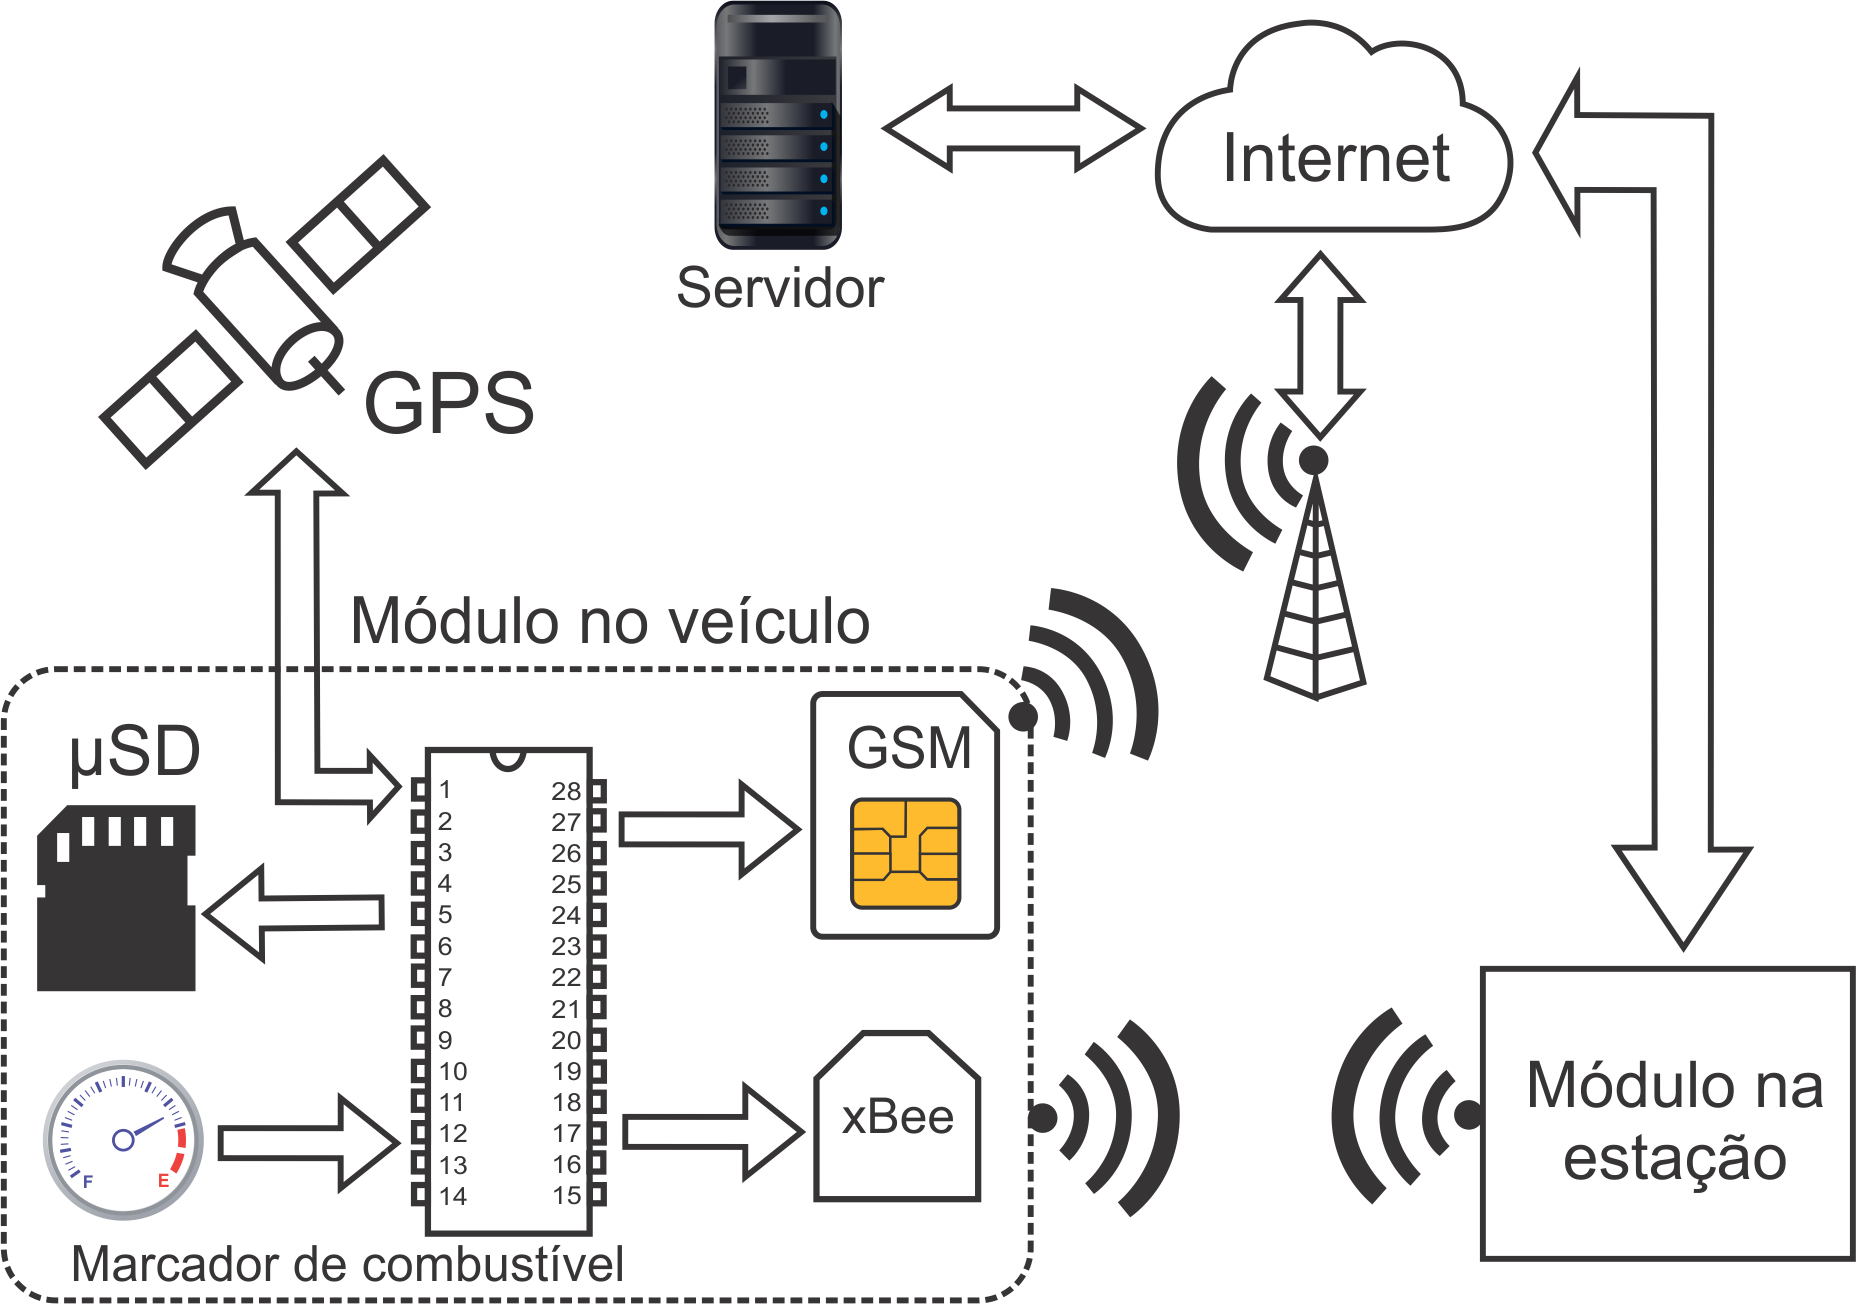
\includegraphics[scale=.8]{ruti1.png}
\label{fig:projeto}
\end{figure}

\chapter{Cronograma de execução}

asdasasdasdd

\bibliography{bibliografia}

\end{document}

